This section will describe the basic design of the \nenwin scheme. Note that \nenwin represents a class of algorithms, similar to neural networks: each network encodes a different algorithm, but the underlying mechanics are the same. Here the underlying mechanics of \nenwin will be explained.

\subsection{Objects}
\nenwin is best described by defining a family of objects known as particles. The scheme uses a subspace of $\mathbb{R}^n$, often $n=2$ is used in this report to support visualizations, but any higher dimensionality can be used as well. Each particle has a position, a velocity and an acceleration, which are all vectors in $\mathbb{R}^n$. Each particle has a mass (i.e. a decimal value, \textit{allowed to be negative}) as well, and its acceleration is at any point in governed by Newton's Second Law \cite{principia} and a force vector $\vec{f}$:
\begin{equation}
    p.acc = \frac{1}{p.mass} \sum_{\vec{f} \text{ acting on } p}\vec{f}
\end{equation}
Where $p.acc$ and $p.mass$ are the acceleration and mass of any particle $p$.

Note that these forces can only be caused by other particles. Each particle has an associated \textit{attraction function}, that describes what force the particle exerts on any other particle. Although many different functions can be used for this purpose, a natural first choice would be the gravity function (with the constant factor $G$ (the gravitational acceleration) replaced by 1):
\begin{equation}
    \norm{\vec{f}} = \frac{p_1.mass \cdot p_2.mass}{\norm{p_1.pos - p_2.pos}^2}. \label{eq:newton_grav_force_norm}
\end{equation}
The direction of the force is the direction from the first particle to the second particle, so the force vector is given by:
\begin{equation}
    \vec{f} = \frac{p_1.pos - p_2.pos}{\norm{p_1.pos - p_2.pos}} \cdot\frac{p_1.mass \cdot p_2.mass}{\norm{p_1.pos - p_2.pos}^2}. \label{eq:newton_grav_force}
\end{equation}

Particles are divided into two general subclasses: Nodes and Marbles. Nodes are used to represent an architecture, they are the fixed part of a \nenwin network that encodes an algorithm. Nodes are further subdivided into MarbleEaterNodes and MarbleEmitterNodes, as described later. Marbles represent input and output data, and are created at runtime. Marbles can keep an optional reference to the datum they represent.

Particles \textit{experience} forces exerted on them by other particles, but also \textit{exert forces onto} other particles. Unlike in classical mechanics, \nenwin does not require these forces to be symmetric. 
To regulate the \textit{experienced} forces, each particle $p$ has the attributes \texttt{marble\_stiffness} and \texttt{node\_stiffness}. These act as multipliers for experienced forces, and are required to be real values in $[0, 1]$.
The forces that each particle $p$ exerts onto other particles, is regulated in a similar way: $p$ has two attributes\texttt{marble\_attraction} and \texttt{node\_attraction}, act as multipliers of the force that $p$ exerts onto other particles. Also these attributes must be real values in $[0, 1]$. 

To summarize, the motion of a particle $p$ is described by the following differential equations:
\begin{align}
    &p.pos = p.pos_0 + \nabla p.pos \cdot t  = p.pos_0 + p.vel \cdot t \label{eq:def_pos} \\
    &p.vel = p.vel_0 + \nabla p.vel \cdot t = p.vel_0 + p.acc \cdot t \label{eq:def_vel}\\
    &\vec{f}_{net}  = \texttt{marble\_stiffness} \cdot \sum_{\text{Mables $m$ acting on $p$}} \frac{p.mass \cdot m.mass}{\norm{p.pos - m.pos}^2} \nonumber \\
    & \qquad + \texttt{node\_stiffness} \cdot \sum_{\text{Nodes $n$ acting on $p$}} \frac{p.mass \cdot n.mass}{\norm{p.pos - n.pos}^2} \label{eq:def_f_net}\\
    &p.acc = \frac{\vec{f}_{net}}{p.mass} \label{eq:def_acc}
\end{align}
Where $t$ denotes the amount of time passed, and $p.pos_0$ and $p.vel_0$ the initial position and velocity respectively of the particle when it was created.
The acceleration of $p$ depends the forces $p$ experiences. These forces are a function of $p$'s relative distances to other Marbles and Nodes (the denominators in \eqref{eq:def_f_net} are distance measures). These distances depend on the value of $p.pos$ and the motion of other particles. Hence $p.pos$, $p.val$ and $p.acc$ are highly dependent on the other particles in a \textsc{Nenwin} model, and can change significantly even when only an very small amount of time passes.

\subsection{MarbleEaterNodes}
To enable output production, a subclass of Node called the \textit{EaterNode} (or more specifically, the \textit{MarbleEaterNode}) is defined: 
each member of this class has a real-valued radius. 
A Marble will be removed from the simulation as soon as the distance between the Marble and any MarbleEaterNode 
becomes smaller than the radius of the MarbleEaterNode: it was 'eaten' by the MarbleEaterNode.
The MarbleEaterNode keeps both a count of the amount of Marbles consumed, 
and a set of references to the associated data of the consumed Marbles.

\subsection{Motivation Emitter Nodes}
\nenwin will have a nonincreasing amount of particles if only Marbles, Nodes and MarbleEaterNode would be used.
Marbles can be removed when eaten by a MarbleEaterNode, 
but the there is no internal way the system can produce new Marbles (other than awaiting new input).
This would imply that the amount of information that can be stored in a \nenwin simulation is also nonincreasing in a \nenwin architecture.

Turing Machines, on the other hand, can \textit{increase} the information stored on their tape.
For example, consider a Turing machine that writes down all binary numbers, 
starting with 0. Let this Turing machine be constructed such that it leaves a blank ('$\Box$') to the left of this 0, 
and then writes the next number (1), and leaves another blank and writes the next number (01), and so on. 
Then if given a tape of only blanks, it will continue to write an infinite amount of binary numbers on it. 
For any reasonable definition of information, 
this would clearly increase the total amount of information on the tape. 

\subsection{EmitterNode}
To make \nenwin able to increase the amount of information, we define an additional particle called the \textit{EmitterNode}
(or, more specifically, a \textit{MarbleEmitterNode}
\footnote{Note that there is no theoretical objection against creating EmitterNodes that emit other Nodes, 
other than the fact that EaterNodes cannot eat each other at the same time.}). 
EmitterNodes are a subclass of MarbleEaterNodes, 
but besides eating they can also (conditionally) create new particles at its own position.

There are many different ways to choose the exact behaviour of MarbleEmitterNodes, but in this paper we use the following:
\begin{itemize}
    \item A MarbleEmitterNode is a special case of a MarbleEaterNode, and tracks also the cumulative mass of Marbles it has consumed in a field \texttt{stored\_mass}.
    \item The MarbleEmitterNodes can only create Marbles with predefined parameters (mass, initial velocity, etc.) \textit{near} its own position.
    \item At a fixed time interval, the MarbleEmitterNode will create a new Marble and subtract its mass from \texttt{stored\_mass}, unless \texttt{stored\_mass} is smaller than the mass of the would-be created Marble. \\
    In case the mass of the Marble is negative, it will only be created as long as the \texttt{stored\_mass} is \textit{at most} the value of the mass of the Marble (i.e. the \texttt{stored\_mass} is also negative, and has a magnitude at least as great as the magnitude of the mass of the Marble).
    \item The created Marble must be within the radius or at an infinitesimal distance from the border of the radius of the MarbleEmitterNode. In case the Marble is within the radius it will be consumed immediately, hence only the infinitesimal distance is a practical option. In implementation, where infinitesimal numbers cannot be represented, a small constant $\epsilon > 0$ can be defined such that we require (if $emitter$ is the MarbleEmitterNode that creates Marble $m$):
    \begin{align}
        emitter.radius < distance(emitter.pos, m.pos) \leq emitter.radius + \epsilon
    \end{align}
	(More informally, MarbleEmitterNodes may only emit Marbles as close to the circumference of their radius as possible, but without immediately eating the Marble again).
\end{itemize}

To see how EmitterNodes can be used to create any arbitrary amount of entropy, consider an EmitterNode that generates Marbles with infinitesimally small mass, or even 0 mass. After eating a Marble with a finite mass, it will be able to generate infinitely many new Marbles. If a dynamic system guides the movement of the Marbles, then each can eventually take on a unique position (since they are not created at the same moment, and the system is dynamic, they will follow a different path). Any information can be encoded in the distribution of these Marbles, which implies that the amount of information in the simulation can be increased in the same way as a Turing Machine can increase the information on its tape.

See \ref{fig:particles_class_diagram} for a diagram the complete particle hierarchy. 

\begin{figure}[h]
    \centering
    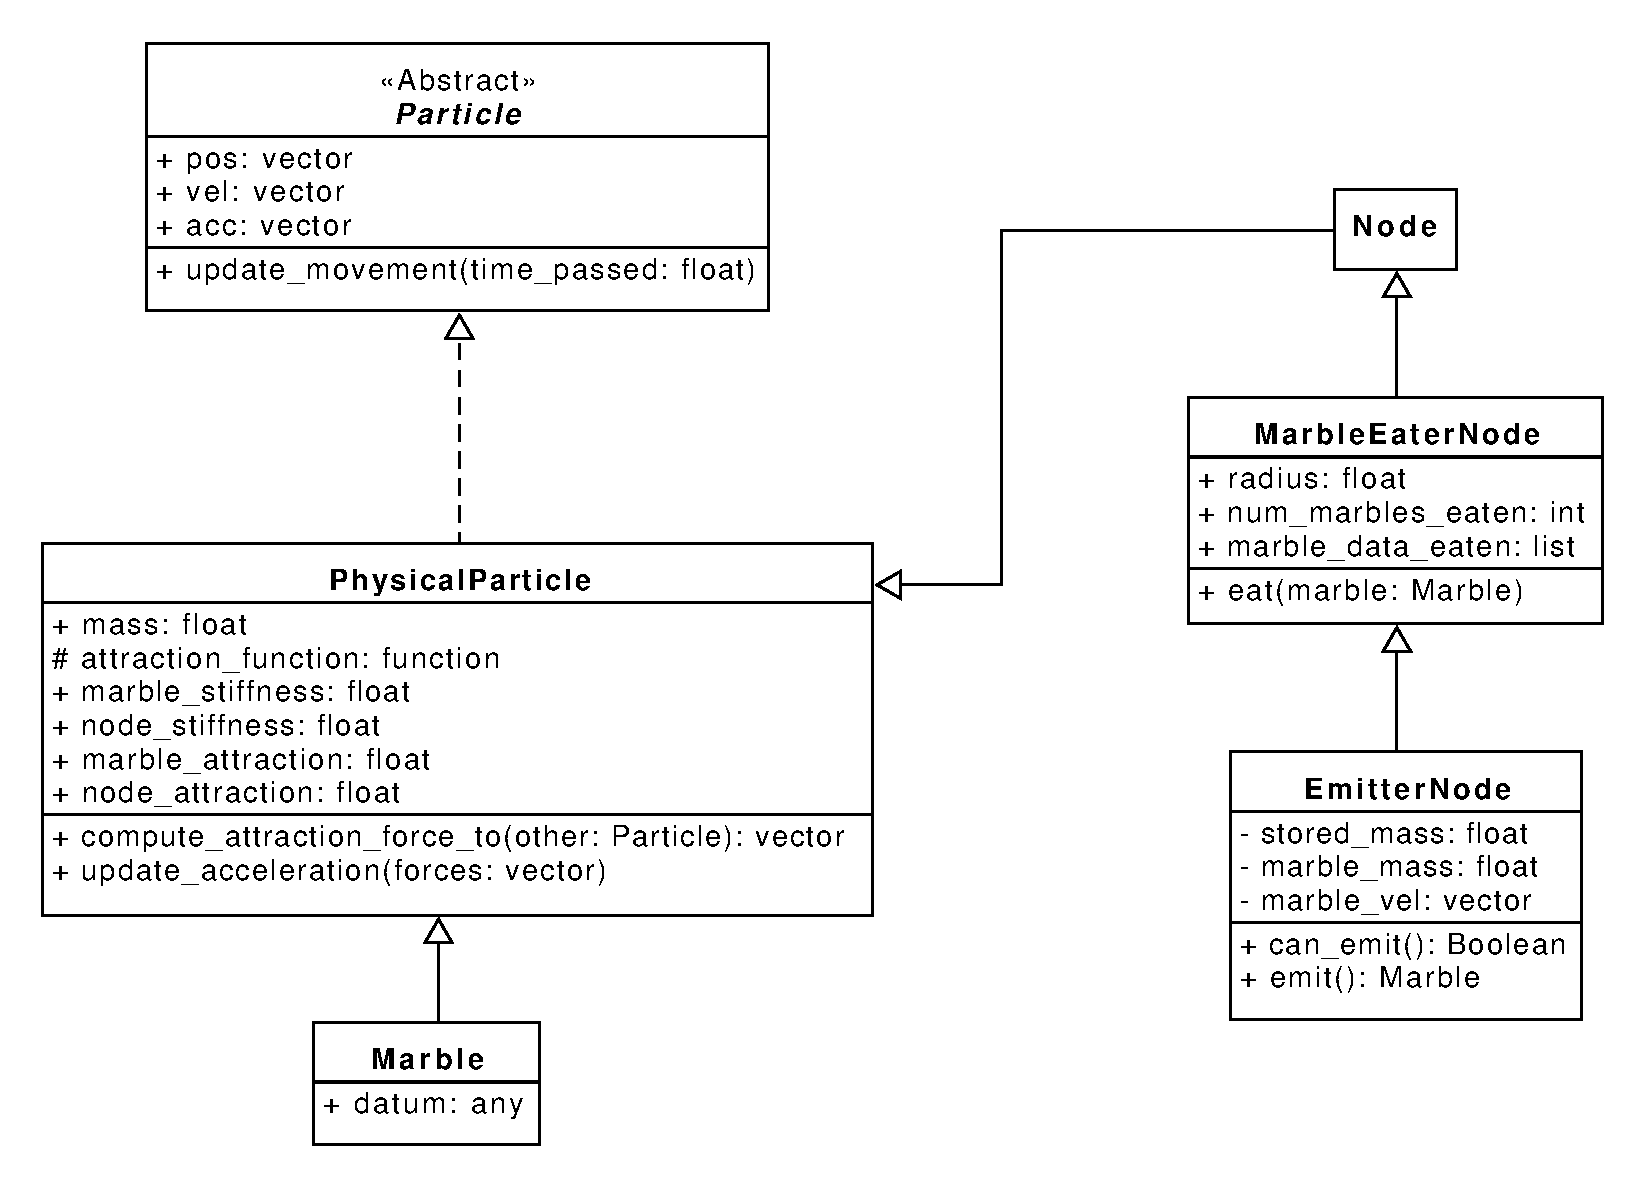
\includegraphics[scale=0.5]{figures/particles_class_diagram.pdf}
    \caption{UML class diagram depicting the inheritance relations between different particles. Note that the exact inheritance and attribute-visibilities may vary between implementations. For example, in the provided implementation, Marble is a subclass of Node.}
    \label{fig:particles_class_diagram}
\end{figure}

\subsection{Particle attributes}
An overview of the different attributes per particle subclass is given in Table \ref{table:attributes}.

\begin{table}[h]
\begin{tabular}{llllll}
\textbf{Attribute} & \textbf{type} & \textbf{Marble} & \textbf{Node} & \textbf{MarbleEaterNode} & \textbf{EmitterNode} \\ \hline
\multicolumn{1}{l|}{\texttt{pos}}                  & \multicolumn{1}{l|}{$\mathbb{R}^n$} & \checkmark & \checkmark & \checkmark & \checkmark \\
\multicolumn{1}{l|}{\texttt{vel}}                  & \multicolumn{1}{l|}{$\mathbb{R}^n$}               & \checkmark & \checkmark & \checkmark & \checkmark \\
\multicolumn{1}{l|}{\texttt{acc}}                  & \multicolumn{1}{l|}{$\mathbb{R}^n$}               & \checkmark & \checkmark & \checkmark & \checkmark \\
\multicolumn{1}{l|}{\texttt{marble\_stiffness}}    & \multicolumn{1}{l|}{{[}0, 1{]}}     & \checkmark & \checkmark & \checkmark & \checkmark \\
\multicolumn{1}{l|}{\texttt{node\_stiffness}}      & \multicolumn{1}{l|}{{[}0, 1{]}}     & \checkmark & \checkmark & \checkmark & \checkmark \\
\multicolumn{1}{l|}{\texttt{marble\_attraction}}   & \multicolumn{1}{l|}{{[}0, 1{]}}     & \checkmark & \checkmark & \checkmark & \checkmark \\
\multicolumn{1}{l|}{\texttt{node\_attraction}}     & \multicolumn{1}{l|}{{[}0, 1{]}}     & \checkmark & \checkmark & \checkmark & \checkmark \\
\multicolumn{1}{l|}{\texttt{attraction\_function}} & \multicolumn{1}{l|}{$f:\mathcal{P}\times\mathcal{P}\rightarrow \mathbb{R}^n$}       & \checkmark & \checkmark & \checkmark & \checkmark \\
\multicolumn{1}{l|}{\texttt{datum}}                & \multicolumn{1}{l|}{any object}     & \checkmark &   &   &   \\
\multicolumn{1}{l|}{\texttt{eaten\_marbles}}       & \multicolumn{1}{l|}{stack of Marbles} &   &   & \checkmark & \checkmark \\
\multicolumn{1}{l|}{\texttt{radius}}               & \multicolumn{1}{l|}{$\mathbb{R}$}           &   &   & \checkmark & \checkmark \\
\multicolumn{1}{l|}{\texttt{stored\_mass}}       & \multicolumn{1}{l|}{$\mathbb{R}$} &   &   & \checkmark & \checkmark \\
\multicolumn{1}{l|}{\texttt{spawnpos}}             & \multicolumn{1}{l|}{$\mathbb{R}^n$}            &   &   &   & \checkmark \\
\multicolumn{1}{l|}{\texttt{prototype\_marble}}    & \multicolumn{1}{l|}{Marble}         &   &   &   & \checkmark
\end{tabular}
\caption{A summary of different attributes used by different particles. $\mathcal{P}$ is used to denote the set of all particles in a given architecture. \newline
Here \texttt{pos}, \texttt{vel} and \texttt{acc} are the position, velocity and acceleration of a particle, which are real vectors defined in $\mathbb{R}^n$ where $n$ is the dimensionality of the architecture. The stiffness and attraction values are real numbers in the interval $[0, 1]$. The attraction function maps two particles to a vector of the same shape as \texttt{acc}.\newline
The \texttt{datum} is any data-element that a Marble represents, and this attribute is allowed to be valueless.\newline
\texttt{eaten\_marbles} is a stack of all Marbles a MarbleEaterNode (or its subclass, a MarbleEmitterNode) has consumed, with the latest consumed Marble on top of the stack. This stack is allowed to be empty. \newline
The \texttt{radius} of a MarbleEaterNode is the maximum distance such that, if a Marble is at this distance or at a smaller distance to the MarbleEaterNode, it will be consumed. \\
The \texttt{stored\_mass} is the cumulative mass of the Marbles in \texttt{eaten\_marbles} of a MarbleEmitterNode, minus the cumulative mass of emitted Marbles. This value is allowed to be negative, which is required to emit negatively-massed Marbles. \newline
The \texttt{spawnpos} is the relative position from the center of an MarbleEmitterNode at which a Marble can be created when emitted, this point is at most \texttt{radius} + $\epsilon$ away from the center of the MarbleEmitterNode, where $\epsilon$ is an infinitesimal number. The prototype Marble is a 'blueprint' of the Marble that is emitted: all its attributes are copied to a new Marble that is being emitted, except the position (which is governed by the combination of the position of the MarbleEmitterNode and \texttt{spawnpos}), the velocity and the acceleration (which are set to $\vec{0}$).}
\label{table:attributes}
\end{table}

\clearpage
\subsection{Application to Machine Learning}
\nenwin is designed to fulfil the role of a decision-making agent, for example as an alternative to neural networks in reinforcement learning or classification tasks. Besides the particle simulation, this would also require the system to receive input and produce output. 

For example, if a \nenwin simulation is used as an agent to play a game, say chess, then it must be able to perceive the current state of the game, and to choose a move to make. As for another example, if a \nenwin simulation is used for an image classification task, then it must be able to read the images, and output a predicted class.

Adding inputs is straightforward: a region in $\mathbb{R}^D$ (where $D$ is the chosen dimensionality of the \nenwin architecture) is chosen as the \textit{input region} $R$. If input datapoints are given in $\mathbb{R}^n$, then one can define a function (an \textit{input placer}) that maps $\mathbb{R}^n$ to a set of Marbles located in $R$. The inputs can be stored in an bi-directional input/output buffer, called a \textit{channel}. The simulation will then check the channel each timestep, and map any data in the channel to Marbles, and insert these into the simulation.

To produce output, MarbleEaterNodes are used. At each timestep, the simulation outputs a vector containing a natural number for each present MarbleEaterNode into the output of the channel. These natural numbers encode the total number of Marbles eaten by each MarbleEaterNode. This vector can, for example, be interpreted as a one-hot encoding for classification (it contains only one '1' when read as soon as the first Marble has been eaten).
For even more detailed output, one can allow external functions to read the exact set of Marbles eaten by each MarbleEaterNode. This latter extension was used for classification training described in a later section.

\subsubsection{Input Placement}
Marbles are used to represent input data, which can either be tabular data, an image, a stream of sound or video, etc.
From the algorithm's side, as described in \ref{alg:Nenwin_V1}, 
this simply means that a new set of Marbles can be added to the simulation at each timestep.
However, it is required to map the input data (together with a designated \textit{input region}) to a set of Marbles first, by means of an \textit{input placer}.
This can be done in very many ways. For example, a datapoint could be used to generate a single Marble, in which the datum is mapped to an attribute of the Marble, such as the position, the mass, the velocity, etc.. It is also possible to use information multiple datapoints to create a single Marble. Furthermore, it is also possible to define a trainable input placer, which can be optimized using marchine learning techniques.

It was chosen to use an input placer (the "GridInputPlacer") that simply spreads the Marbles evenly in a grid over the input region (in order of the input vector, from left to right, top to bottom). This input placer creates a Marble for each datapoint.
Note that this choice is rather arbitrary: as of current there are no arguments why aligning the Marbles in another pattern (such as on a circle) would be less effective.

Two variants of the GridInputPlacer were used:
\begin{itemize}
	\item MassInputPlacer: maps each datapoint to a Marble, whose mass is set to the value of the datapoint. The velocity is set to $\vec{0}$.
	\item VelInputPlacer: maps each datapoint to a Marble, whose velocity is set to a vector of which each element equals the value of the datapoint. It sets the mass of each Marble to 1.0.
\end{itemize}

All variants set, for each Marble, the remaining attributes as follows:
\begin{itemize}
	\item the radius of the threshold radius to 100.
	\item the acceleration to $\vec{0}$.
	\item the \texttt{marble\_stiffness} to 1.
	\item the \texttt{node\_stiffness} to 0.
	\item the \texttt{marble\_attraction} to 0
	\item the \texttt{node\_attraction} to 1.
\end{itemize}



\subsubsection{Simulation}
See Algorithm \ref{alg:Nenwin_V1} below for an abstract pseudocode description how a \nenwin can be simulated. This pseudocode includes input-output handling. Note that in implementation the functionality will be subdivided into different modules. 
It is for example equally fast, but from an Object-Oriented point of view preferable, to first create Marble instances for new inputs and then sending them over the channel rather than sending the raw data itself. This does not affect the behaviour of the algorithm.

\begin{algorithm}[h]
	\caption{\\\textsc{Nenwin}\textnormal{\texttt{(nodes, input\_space, placement\_function, mass\_function, channel, attraction\_function)}}}
	\label{alg:Nenwin_V1}
	\newcommand{\dataStyle}[1]{\textbf{\texttt{#1}}}
	\SetAlgoLined
	\SetKwSty{texttt}
	\SetDataSty{dataStyle}
	% Setup variables
	\SetKwData{nodes}{nodes}
	\SetKwData{input}{input\_space}
	\SetKwData{placement}{input\_placer}
	\SetKwData{channel}{channel}
	\SetKwData{node}{Node}
	\SetKwData{grav}{attraction\_function}
	\SetKwData{mass}{mass\_function}
	\SetKwData{eaters}{eater\_nodes}
	\SetKwData{emitters}{emitter\_nodes}
	% Input and output
	\KwIn{
		\nodes: A set of \node objects, each having a position, velocity and acceleration in $\mathbb{R}^D$ and a stiffness and a mass in $\mathbb{R}$.\\
		\input: A (hyperrectangular) subspace of $\mathbb{R}^D$.
		\placement: A function that maps input vectors (in $\mathbb{R}^n$) to Marbles located in \input.\\
		\channel: A bi-directional communication channel over which any finite real-valued vectors can be sent.\\
		\grav: A function that maps two Marbles (usually using their masses and their relative distance) to an attraction force vector.		
	}
	\KwOut{\texttt{None}}
	$particles \leftarrow \nodes$ \;
	$\eaters \leftarrow [node: node \in \nodes \land node \text{ is a } \textsc{MarbleEaterNode}]$ \;
	\tcc{The following is a subset of 'eaters':}
	$\emitters \leftarrow [node: node \in \nodes \land node \text{ is a } \textsc{MarbleEmitterNode}]$ \;
	\While{\texttt{True}}{
		\If{there is input on the channel}{
			\For{$\vec{v} \in \channel$}{
				$particles \leftarrow particles \cup \{\placement(\vec{v})\}$\;
			}
		}
		\If{there is an output request on the channel}{
			$output \leftarrow \text{ a new empty list}$ \;
			\For{$node \in \eaters$}{
			    $output.append(node.num\_marbles\_eaten)$ \;
			}
			Place $output$ on the channel \;
		}
		\For{$p \in particles$}{
			$\vec{f} \leftarrow \sum_{o \in particles \setminus\{p\}} \frac{o.pos - p.pos}{\doublenorm{o.pos - p.pos}} \cdot \grav(p, o)$ \;
			\tcc{Newton's Second Law}
			$p.acc \leftarrow p.mass \cdot \vec{f}$ \;
		}
		\For{$e \in \emitters$}{
		    \If{$\norm{e.stored\_mass} \geq \norm{e.prototype\_marble.mass} \land \sgn{e.stored\_mass} = \sgn{e.prototype\_marble.mass}$}{
		    $particles \leftarrow particles \cup (\text{a copy of $e.prototype\_marble$ at position $e.pos + e.spawnpos$})$
		    }
		}
		\For{$particle \in particles$}{
			Compute and update $particle$'s next position and velocity given their current acceleration (using numerical integration). \;
		}
		\For {$marble \in particles \setminus nodes$}{
			\For{$node \in \eaters$}{
				\If{$distance(marble.pos, node.pos) \leq node.radius$}{
					$particles \leftarrow particles \setminus \{marble\}$ \;
					$node.stored\_mass \leftarrow node.stored\_mass + marble.mass$ \; $node.eaten\_marbles \leftarrow node.eaten\_marble \cup \{marble\}$\;
				}
			}
		}
		}
\end{algorithm}

\clearpage